
\chapter{Técnicas de visualização de dados em \emph{CBIR}}

Um problema dos algoritmos empregados na extração de características do contorno das formas, que foram abordados no Capítulo \ref{chap:contour}, é a elevada dimensionalidade da representação vetorial obtida. Além de dificultar compreender a organização dos dados, a elevada dimensionalidade acarreta em maior complexidade do sistema computacional que deve lidar com essa informação. 

Através de técnicas de redução de dimensionalidade é possível gerar visualizações gráficas dos dados, o que permite compreender melhor sua estrutura. Ademais, tais técnicas removem informações redundantes e irrelevantes, reduzindo assim a complexidade da representação obtida.

Apresentamos neste capítulo duas técnicas de visualização de dados que foram empregadas neste trabalho na avaliação da capacidade discriminativa dos descritores do contorno de formas: a análise das componentes principais (\emph{PCA}) e o mapa auto-organizável de Kohonen (SOM).

Pelo fato dessas técnicas requererem que os vetores de características das formas sejam de mesma dimensão, e por empregarem como medida de similaridade a distância euclidiana, essas técnicas foram aplicadas aos descritores energia de dobramento multiescala e dimensão fractal multiescala.

%Essas técnicas tem em comum a propriedade de projetar os dados de dimensionalidade elevada em um espaço bidimensional. 

\section{Análise das componentes principais (PCA)}

\begin{figure}[h!]
  \caption{\label{fig:nuvem_pca} Ilustração geométrica do método de obtenção da assinatura de sequência de ângulos.}
  \centering
  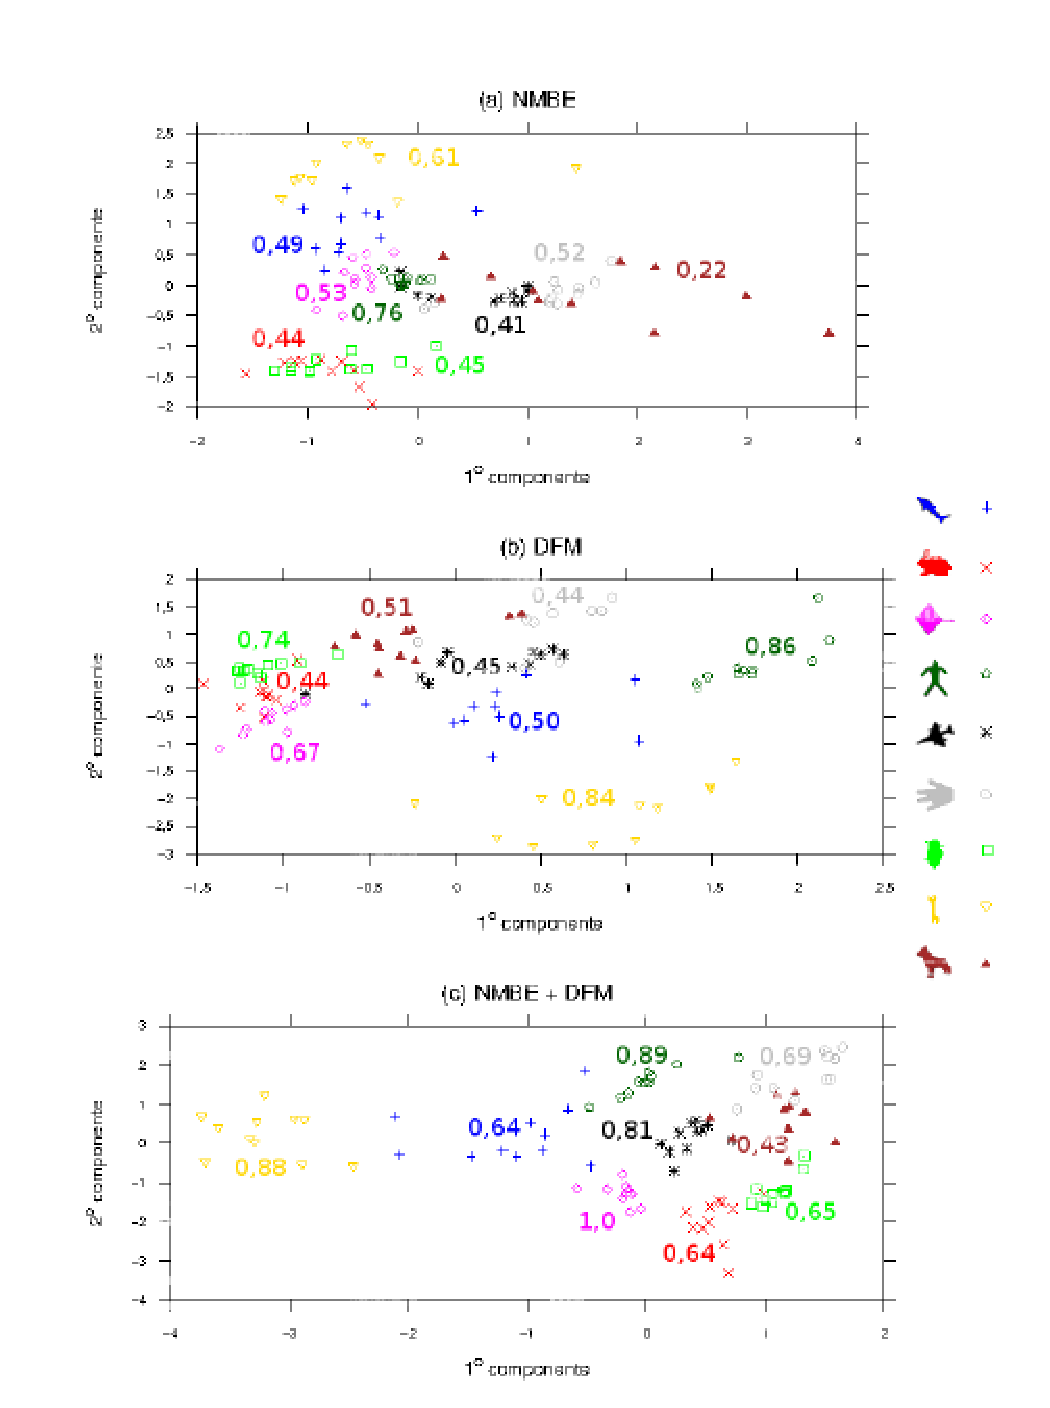
\includegraphics[width=0.75\textwidth]{nuvem_pca.eps}
\end{figure}

O propósito da análise das componentes principais é obter um conjunto de variáveis não correlacionadas, em ordem decrescente de importância, a partir da combinação linear das variáveis originais. Sob o aspecto geométrico, esse processo de combinar linearmente as variáveis pode ser entendido como realizar a rotação dos eixos do sistema de coordenadas original, a fim de se encontrar um novo sistema de coordenadas ortogonal em que as variáveis transformadas apresentem máxima variância. 

Desde que a maior parte da variância esteja concentrada nas primeiras componentes das variáveis transformadas, consegue-se obter através dessa técnica uma representação com um número reduzido de variáveis.

A técnica \emph{PCA} é não supervisionada, pois não leva em consideração informação a priori dos agrupamentos, ou rótulos, dos dados.  

Sendo a transformação \emph{PCA} linear, temos que

\begin{equation}\label{eq:PCA1}
\mathbf{y}=\mathbf{A}^T\mathbf{x}
\end{equation}

, aonde $ \mathbf{A} = \begin{pmatrix}
  a_{1,1} & a_{2,1} & \cdots & a_{p,1} \\
  a_{1,2} & a_{2,2} & \cdots & a_{p,2} \\
  \vdots  & \vdots  & \ddots & \vdots  \\
  a_{1,p} & a_{2,p} & \cdots & a_{p,p}
 \end{pmatrix} = 
 \begin{pmatrix}
 \mathbf{a_{1}}&
 \mathbf{a_{2}}&
 \cdots&
 \mathbf{a_{p}}
 \end{pmatrix}$ é a matriz de tranformação, $\mathbf{x} = \begin{pmatrix} x_1&x_2&\ldots&x_p\end{pmatrix}^T$ e $\mathbf{y} = \begin{pmatrix}y_1&y_2&\ldots&y_p\end{pmatrix}^T$ vetores de variáveis aleatórias e $\mathbf{a_1}\text{ a }\mathbf{a_p}$ vetores dos coeficientes da base de transformação.
 
Logo, cada variável de saída $y_i$ é obtida através da combinação linear das variáveis de entrada pela seguinte equação:
 
 \begin{equation}\label{eq:PCA2}
 y_i = \sum\limits_{j = 1}^p a_{i,j}x_j = \mathbf{a_i}^T\mathbf{x}
 \end{equation}

Pode-se demonstrar que, para se obter em $\mathbf{y}$ variáveis que não são correlacionadas,  deve-se atribuir aos vetores de coeficientes $\mathbf{a_1} \ldots \mathbf{a_p}$ os auto-vetores da matriz de covariância de $\mathbf{x}$, sendo esta última dada por: 

\begin{equation}\label{eq:PCA3}
\mathbf{\Sigma_x} = E{[\mathbf{xx}^T]}-E{[\mathbf{x}]}E{[\mathbf{x}^T]}
\end{equation}

 aonde $E[.]$ denota o operador esperança. 
Já que $\mathbf{\Sigma_x}$ é de dimensão $p \times p$, temos associada a esta $p$ auto-vetores ($\mathbf{a_1}\text{, }\mathbf{a_2}\text{, }\ldots\text{, }\mathbf{a_p}$) com $p$ auto-valores ($\lambda_1 > \lambda_2 \ldots > \lambda_p$) correspondentes, sendo cada auto-valor $\lambda_i$ a variância de cada variável de saída $y_i$ obtida através da Equação \ref{eq:PCA2}. 

Selecionando dentre as componentes somente aquelas de maior variância, que implica em construir a matriz de transformação apenas com os auto-vetores mais significativos, é possível obter uma representação dos dados em um espaço de dimensão reduzida e de mais fácil entendimento do ponto de vista geométrico.

Na figura \ref{fig:nuvem_pca} temos representadas as projeções das duas componentes principais de maior variância para cada um dos descritores avaliados. Os valores numéricos correspondem a taxa de acerto média nos experimentos de recuperação de formas pelo conteúdo alcanças para cada classe de formas representada.

\section{Mapa auto-organizável de Kohonen}

O mapa auto-organizável de Kohonen, ou rede \emph{SOM} \cite{Kohonen:2001}, consiste em um tipo de rede neural de aprendizagem não supervisionada. Desenvolvida por \citeonline{Kohonen:1982}, a rede \emph{SOM} projeta os vetores apresentados em sua entrada de um espaço N-dimensional para um espaço bidimensional, preservando a estrutura topográfica do espaço vetorial de origem. Em outras palavras, se dois vetores encontram-se próximos no espaço de entrada, estes preservarão essa relação de proximidade no espaço de projeção. 

\begin{comment}
Em seu processo de treinamento, a rede \emph{SOM} agrupa os vetores de entrada através de um processo de aprendizado competitivo mantendo a estrutura topológica do espaço vetorial de entrada.
\end{comment}

Sendo uma ferramenta para análise exploratória de dados, esse tipo de rede neural tem sido empregada para visualização de imagens \cite{Strong2011774}, identificação de agrupamentos \cite{Kuroiwa200031}, classificação de texturas \cite{595364}, bem como outras aplicações.

\citeonline{Ultsch:1990} demonstraram que, embora a rede \emph{SOM} organize os vetores em agrupamentos, esta não representa as distâncias entre os mesmos de maneira fidedigna. Isso torna a análise direta do mapa de projeções não adequada para a análise dos agrupamentos estabelecidos. 

Para contornar esse problema, os referidos autores desenvolveram um método bidimensional de representação conhecido como matriz unificada de distâncias ou matriz-U. Obtida a partir do mapa \emph{SOM} essa matriz mostra, preservando a topologia, a relação de distância entre as estruturas mapeadas \cite{Ultsch:1990}. 

\section{Método de avaliação da capacidade discriminativa dos descritores}

A Figura \ref{fig:metodo_4} ilustra o método que emprega visualização dos dados na avaliação da capacidade discriminativa dos descritores de formas.

\begin{figure}[h!]
  \caption{\label{fig:metodo_4} Método de avaliação de descritores multiescala do contorno de formas. (a) Base de imagens. (b) Extração de características. (c) Descritores de formas. (d) Análise de similaridade a partir da matriz-U. (e) Avaliação de agrupamentos a partir da medida silhouette.}
  \centering
  \includegraphics[width=0.75\textwidth]{metodo_v4.png}
\end{figure}

O primeiro passo consiste em realizar a extração de características num conjunto de formas binárias rotuladas (Figura \ref{fig:metodo_4}a e Figura \ref{fig:metodo_4}b através do método sob análise. Disso resulta um conjunto de descritores, ou vetores de características (Figura \ref{fig:metodo_4}c). 

A avaliação de qualidade dos descritores se dá de forma qualitativa e quantitativa. Na metodologia de avaliação qualitativa (Figura \ref{fig:metodo_4}d) é utilizada a rede auto-organizável de Kohonen para obtenção da matriz de distâncias unificada, ou matriz-U. Essa última é empregada como ferramenta de visualização dos dados, o que possibilita a análise dos agrupamentos das formas produzido pelo método de descrição sob avaliação. A metodologia de avaliação quantitativa (Figura \ref{fig:metodo_4}e) calcula a medida de avaliação de agrupamentos \emph{Silhouette} aos vetores que representam as amostras das formas.

% Then, our approach accomplishes yielding a visual similarity map. This map provides a graphical representation that supports cluster analysis and visualization and, furthermore, it illustrates how shape description spatially organizes shapes in a two-dimensional projection space.  

%The quantitative evaluation methodology (Figure \ref{fig:Avaliacao}e) applies the \emph{Silhouette} measure \citep{Rousseeuw:1987} to the labeled shape samples and calculates \emph{Silhouette} values for both multiscale shape descriptors. Then, it computes the average \emph{Silhouette} per class which indicates the ability of each descriptor to discriminate shapes that belong to different classes.

%It is worth noting that both evaluation methodologies rely on a similarity measure to compare shape feature vectors.  In fact, our approach deals with feature vectors of same dimension and therefore we adopt the $L_2$ norm, i.e.,  the Euclidean norm as the similarity measure. 

\section{Resultados Experimentais}

Os experimentos de avaliação de desempenho dos descritores produziram como saída as matrizes-U que estão apresentadas na Figura \ref{fig:nmbe_som_map}, Figura \ref{fig:mfd_som_map} e  Figura \ref{fig:som_kimia_216}. Estes resultados mostram que as regiões delimitadas com linhas tracejadas, nas Figura \ref{fig:nmbe_som_map} e Figura \ref{fig:mfd_som_map}, correspondem as classes de formas com os maiores valores médios da medida Silhouette (Figura \ref{fig:silhouette} (a) e Figura \ref{fig:silhouette} (b)). Desta forma, pode-se deduzir que ambos os descritores foram capazes de caracterizar estas classes de formas corretamente.

Já os grupos delimitados com linhas contínuas nas referidas Figuras referem-se a classes de formas com os menores valores de Silhouette média. De fato, estas formas aparecem nas matrizes-U dispersas em sub-grupos, o que implica que ambos os descritores falharam em caracterizar as formas destas classes.
  
As Figuras \ref{fig:dude_tool_mfd} e \ref{fig:dude_tool_nmbe} mostram objetos das classes de formas de humanos e ferramentas. Ambos os descritores foram capazes de discriminar os objetos das referidas classes como evidenciado nos gráficos apresentados. As matrizes-U (Figuras \ref{fig:nmbe_som_map} e \ref{fig:mfd_som_map}) também confirmam esse resultado exibindo, para essas classes de formas, homogeneidade intra-classe e separabilidade inter-classes.

\begin{comment}
Figure \ref{fig:descritores} displays objects (human and tool shapes) for which the \emph{NMBE} and \emph{MFD} descriptors are able to reliably discriminate subtle differences among them and, furthermore, their respective U-matrices confirm this ability. 
The U-matrices (Figures \ref{fig:projkimia99}a and \ref{fig:projkimia99}b) exhibit an intra-class homogeneity and a high separability between these classes. Thus, we conclude that these shape descriptions are intuitive and effective representations for pattern recognition and CBIR applications.

Regarding the human shapes, the  \emph{MFD} descriptor presents greater dispersion in the U-matrices (Figure \ref{fig:projkimia99_dfm}) than \emph{NMBE} (Figure \ref{fig:projkimia99_en}). And this is consistent with the \emph{Silhouette} measure,  which value for human shapes described by \emph{MFD} is lower than the one obtained from \emph{NMBE}.

Moreover, the closely-spaced signals (dotted red and solid blue lines) in Figure \ref{fig:descritores}a that describe  tool and human shapes show that \emph{NMBE} is more robust to subtle local differences than \emph{MFD} within classes. On the other hand, Figure \ref{fig:descritores}b illustrates the weak discriminating property of \emph{MFD} within classes.

Actually, the small variation of \emph{NMBE} within classes and the large variation of it for objects which belong to different classes are in line and consistent with U-matrix information in Figure \ref{fig:projkimia99}. 
 
\color{red}
In these graphs, the shapes whose descriptions follow the same pattern appear close to each other in the U-matrix, whereas the shapes which descriptions are more dispersive of the pattern are mapped in the U-matrix far away of its corresponding group. Specific examples of the latter condition are the human shapes numbered as $2$ and $4$ in Figures \ref{fig:descritores}a and \ref{fig:descritores}b respectively.
\color{black}
To describe human shapes, the  \emph{MFD} descriptor presents greater dispersion in the U-matrices (Figure \ref{fig:projkimia99_dfm}) than the \emph{NMBE} descriptor (Figure \ref{fig:projkimia99_en}). The  silhouette explains this behavior, since for humans its value is lower to the \emph{MFD} descriptor than the value to the \emph{NMBE} descriptor.

Furthermore, there is a larger variation among tools descriptions in the graphs of  the figure \ref{fig:descritores}a than the  variations observed in the graphs of the figure \ref{fig:descritores}b. Coherently, the corresponding shapes appears in the U-matrix more dispersed  for the \emph{MFD} description than for the \emph{NMBE} description.
\end{comment}

\begin{figure}[h!]
  \caption{\label{fig:nmbe_som_map} Matriz-U para as formas da base Kimia99 representadas com o descritor Energia de dobramento multiescala.}
  \centering
  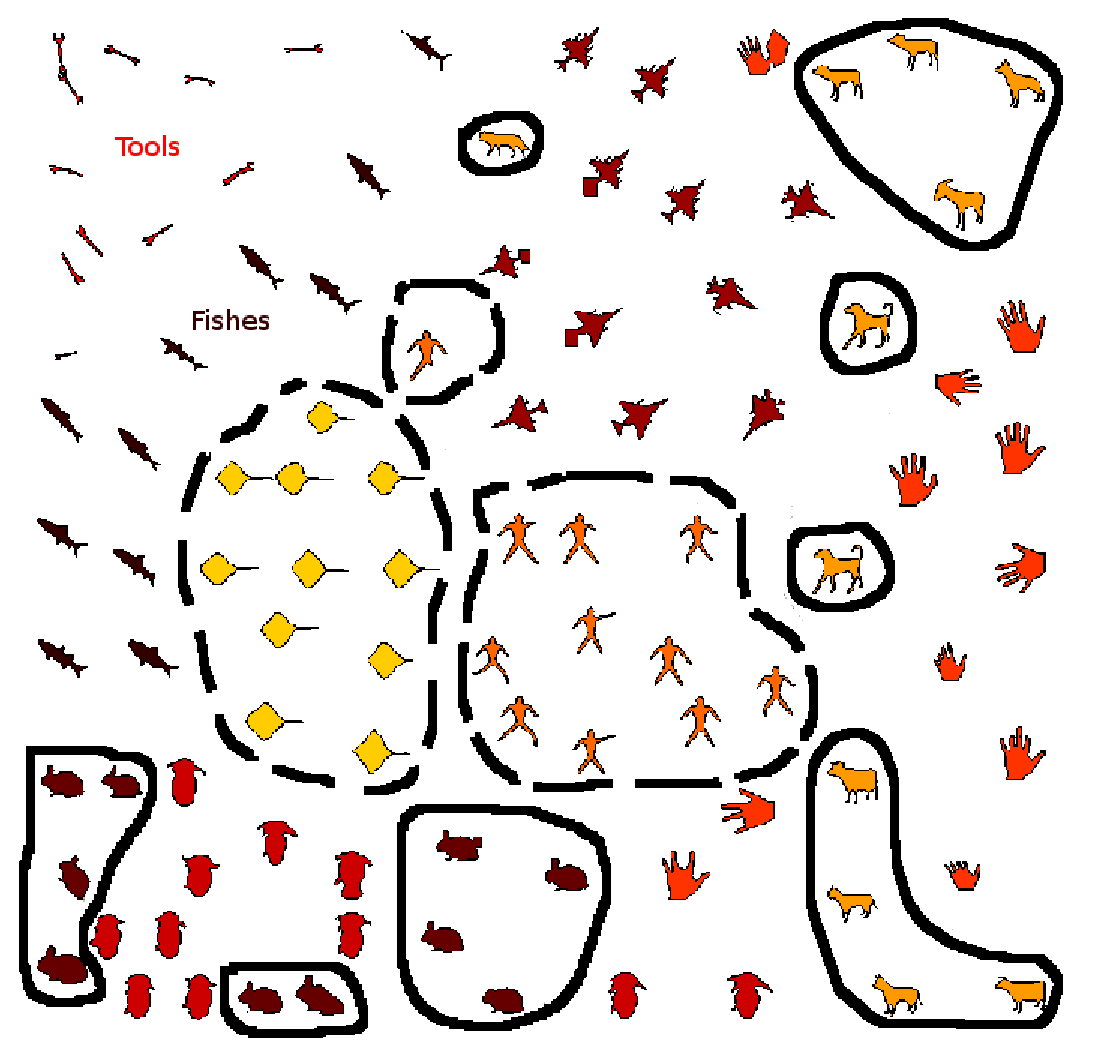
\includegraphics[width=0.5\textwidth]{nmbe_som_map_v4.eps}
\end{figure}

\begin{figure}[h!]
  \caption{\label{fig:mfd_som_map} Matriz-U para as formas da base Kimia99 representadas com o descritor Dimensão fractal multiescala.}
  \centering
  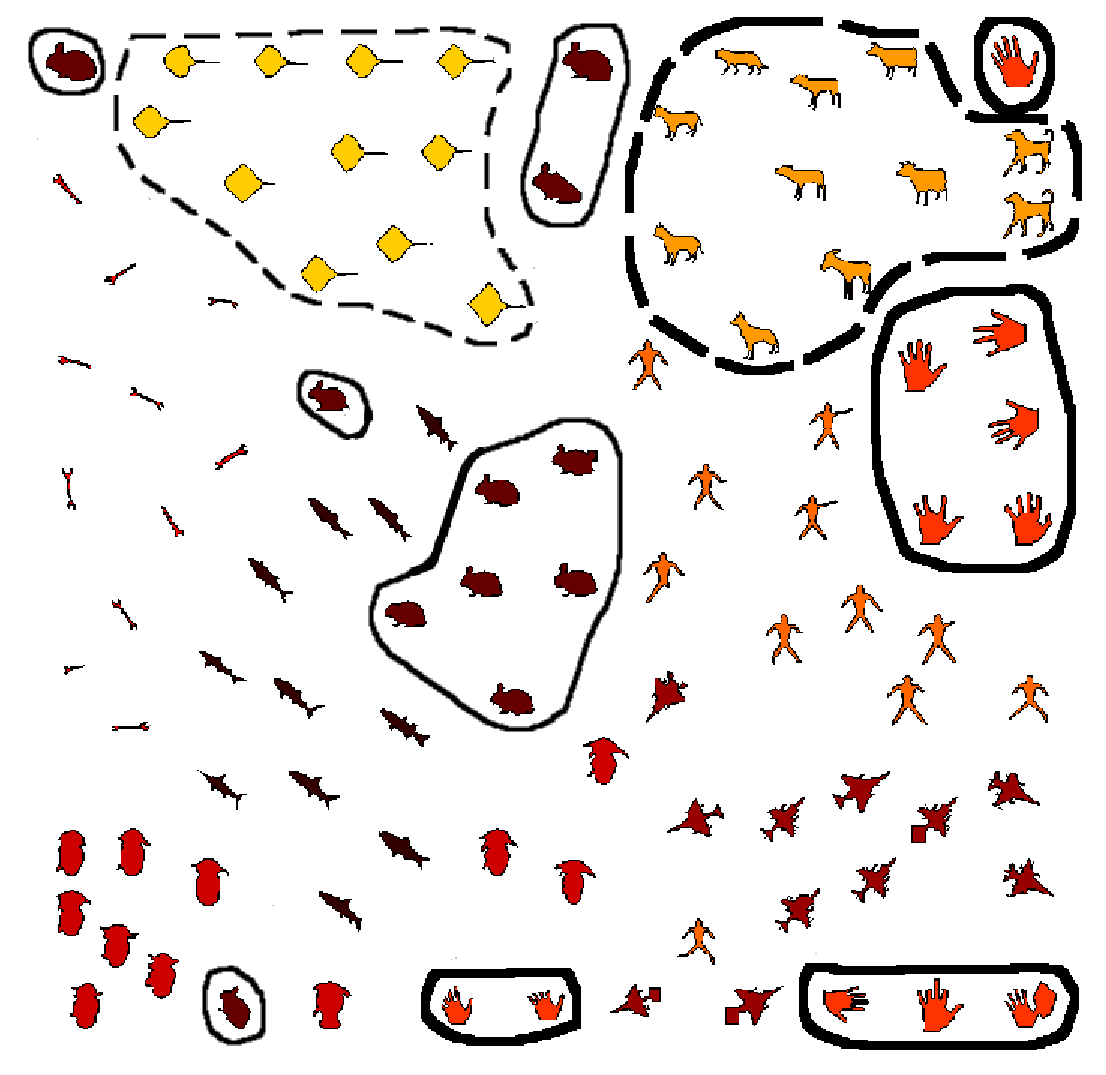
\includegraphics[width=0.5\textwidth]{mfd_som_map_v3.eps}
\end{figure}
  
\begin{figure}[h!]  \caption{\label{fig:som_kimia_216} Para o descritor energia de dobramento multiescala e a base Kimia-216: (a) Matriz-U. (b) Alguns resultados de recuperação de formas pelo conteúdo.}
  \centering
  \includegraphics[width=0.5\textwidth]{retr_som_kimia216_v2.png}
\end{figure}

\begin{figure}[h!]
  \caption{\label{fig:silhouette} Silhouette média por classe aferida nos experimentos de recuperação de formas pelo conteúdo, com a base Kimia-99, para os descritores (a) Dimensão fractal multiescala; (b) Energia de dobramento multiescala.}
  \centering
  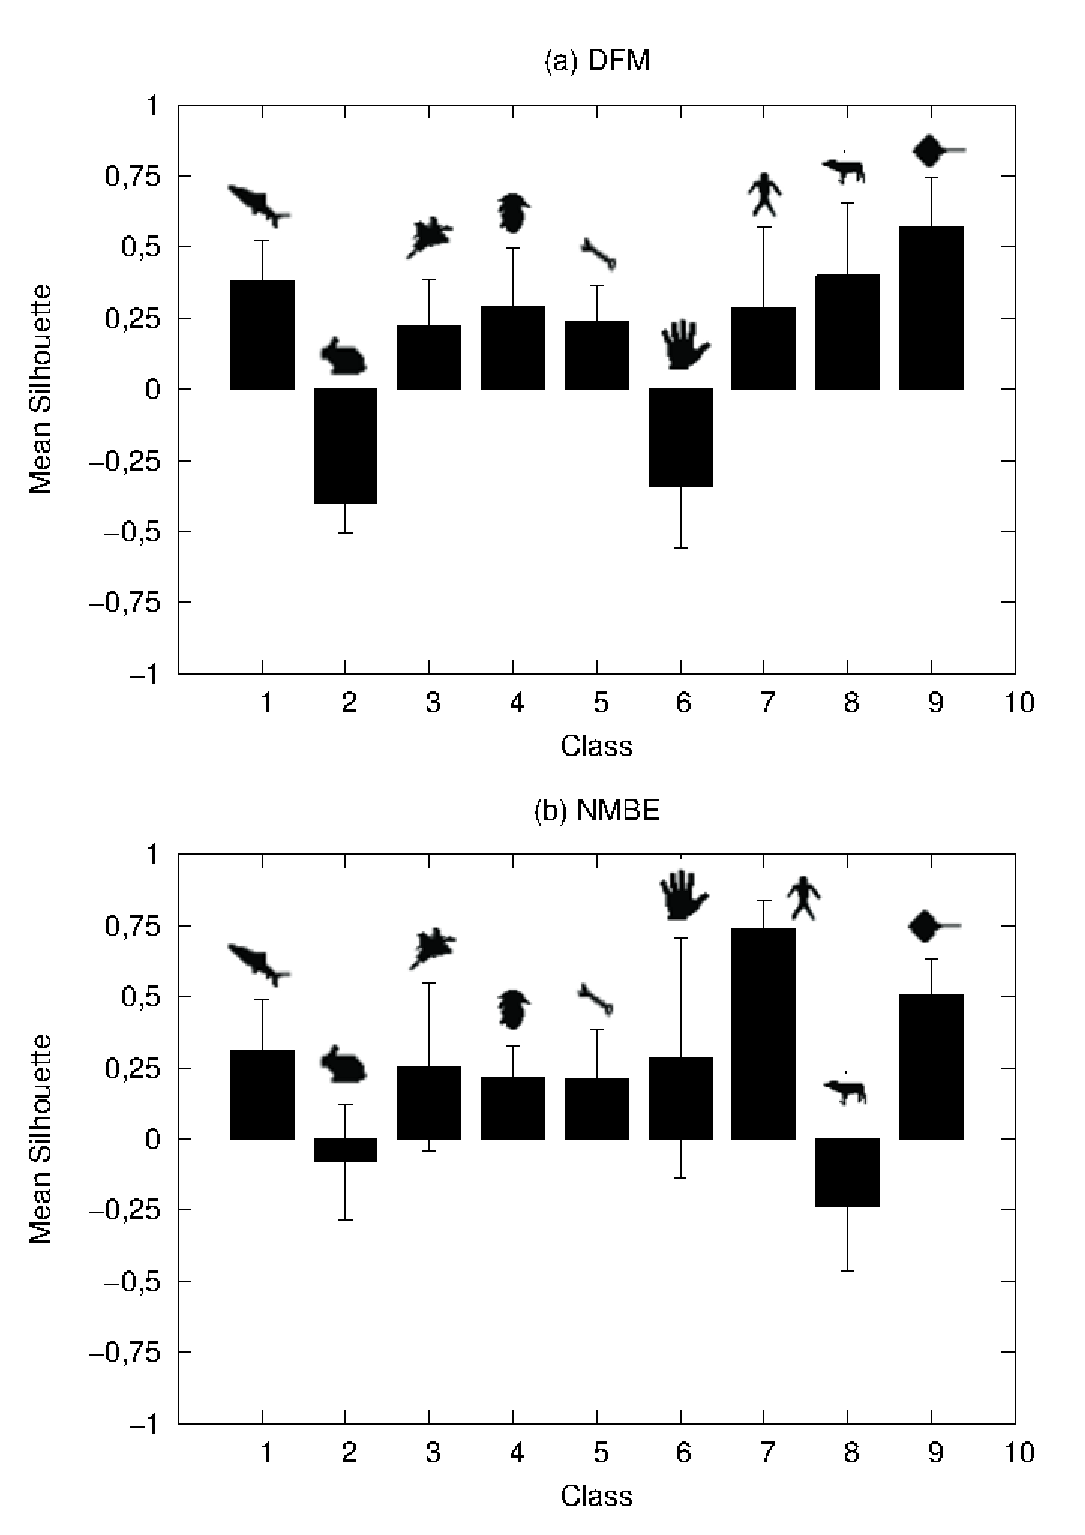
\includegraphics[width=0.5\textwidth]{resultado_silhouette.eps}
\end{figure}

\begin{figure}[h!]
  \caption{\label{fig:dude_tool_mfd}   Vetores de características calculados para amostras das formas de humanos e de ferramentas com o descritor dimensão fractal multiescala.}
  \centering
  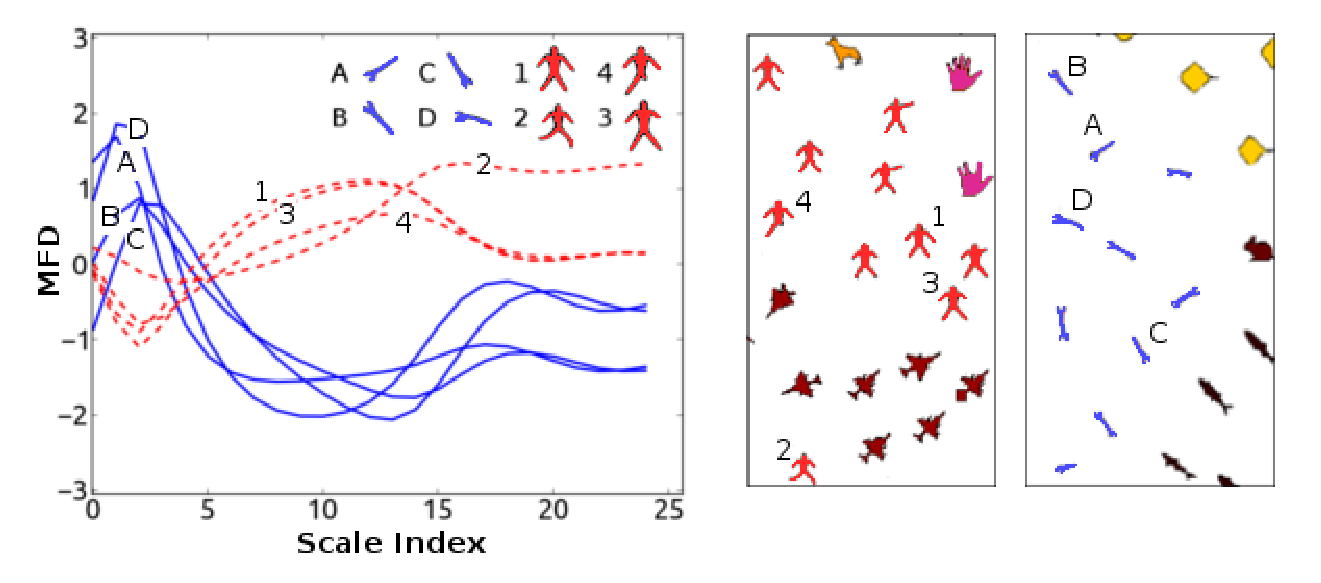
\includegraphics[width=0.75\textwidth]{dude_tool_mfd_v6.eps}
\end{figure}

\begin{figure}[h!]
  \caption{\label{fig:dude_tool_nmbe} Vetores de características calculados para amostras das formas de humanos e de ferramentes com o descritor energia de dobramento multiescala.}
  \centering
  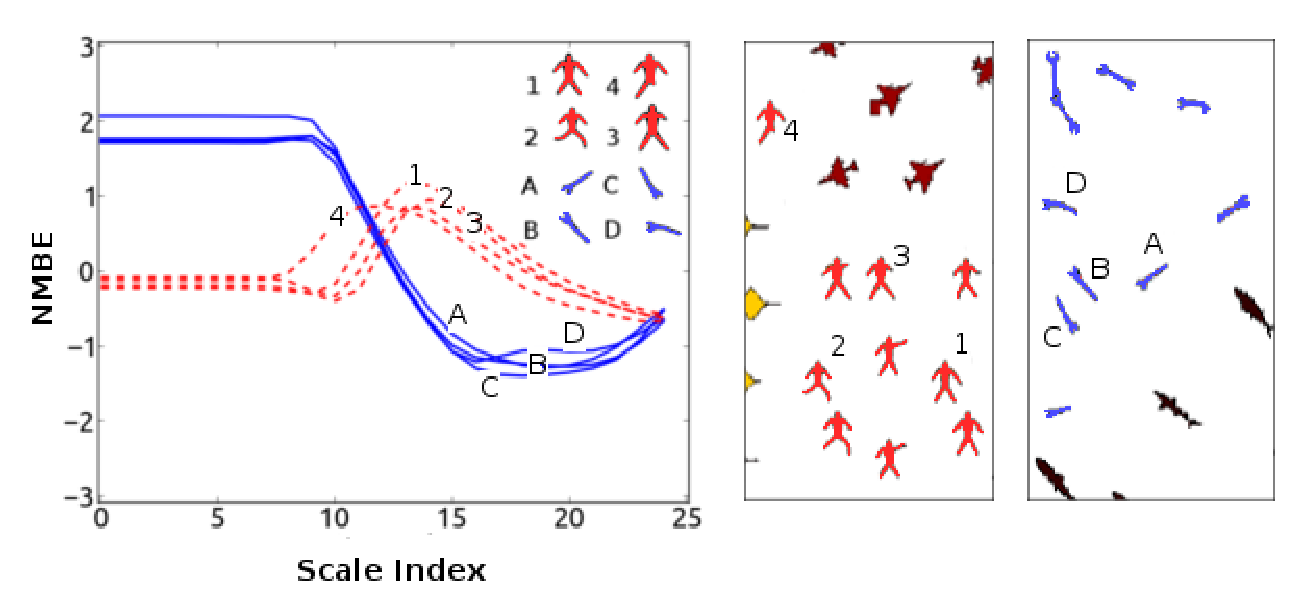
\includegraphics[width=0.75\textwidth]{dude_tool_nmbe_v6.eps}
\end{figure}


\begin{comment}
\begin{figure}[h!]
  \caption{\label{fig:som_nmbe} Visualização dos dados obtida com o mapa auto-organizável de Kohonen para a descrição \emph{NMBE}.}
  \centering
  \includegraphics[width=0.5\textwidth]{mapa_som_descritor_nmbe.png}
\end{figure}

\begin{figure}[h!]
  \caption{\label{fig:som_dfm} Visualização dos dados obtida com o mapa auto-organizável de Kohonen para a descrição \emph{NMBE}.}
  \centering
  \includegraphics[width=0.5\textwidth]{mapa_som_descritor_dfm.png}
\end{figure}
\end{comment}

\chapter{Teoria da informação em recuperação de formas}

%Um dos desafios no campo de visão computacional é fazer com que computadores avaliem o grau de similaridade existente entre formas extraídas de imagens. Embora não esteja completamente elucidado como os sistemas de visão biológicos realizam tal tarefa, busca-se para esta finalidade obter medidas de similaridade que operem de forma fidedigna aos sistemas de visão biológicos. 

Conceitos da teoria da informação têm sido aplicados, recentemente e com sucesso,  em problemas de visão computacional e reconhecimento de padrões. Isso porque tais conceitos têm se mostrado apropriados para a modelagem do comportamento dos sistemas biológicos de percepção visual. \cite{Escolano:2009}. 

Um desses conceitos é o de divergência estocástica. Com aplicações em probabilidade e estatística, processamento de sinais, reconhecimento de padrões e teoria da informação,  divergentes são medidas de similaridade entre distribuições de probabilidades. 

\begin{comment}
From Sample Similarity to Ensemble
Similarity: Probabilistic Distance Measures
in Reproducing Kernel Hilbert Space


Probabilistic distance measures find use in many research
areas such as probability and statistics, pattern recognition,
information theory, communication, and so on. In statistics,
the probabilistic distances are often used in asymptotic
analysis. In pattern recognition, pattern separability is
usually evaluated using probabilistic distance measures [1],
[2] such as Chernoff or Bhattacharyya distances because they
provide bounds for the probability of error. 
\end{comment}

Neste capítulo apresentamos como tais medidas podem ser aplicadas na avaliação de similaridade entre formas, com base em suas assinaturas, no contexto de aplicações de recuperação de formas pelo conteúdo.

\section{Divergentes e similaridade entre formas}

A avaliação de similaridade entre formas a partir de medidas de divergência requer que as informações das assinaturas, abordadas na Seção \ref{sec:Assinatura} do Capítulo \ref{chap:contour}, sejam tratadas como variáveis aleatórias e que suas distribuições de probabilidade sejam estimadas. 

Está ilustrado na  Figura \ref{fig:metodo_distancia} como divergentes podem ser aplicados na avaliação da similaridade entre duas formas A e B. No método em questão, as distribuições de probabilidade de quatro assinaturas distintas dos contornos das formas são estimadas, através de histogramas, para em seguida calcular as medidas de divergência. 

Uma medida de similaridade é então obtida  a partir da média ponderada das medidas de divergência.

\begin{figure}[h!]
  \caption{\label{fig:metodo_distancia} Método para avaliação da similaridade entre duas formas A e B utilizando distância estocástica e histogramas das assinaturas do contorno das formas.}
  \centering
  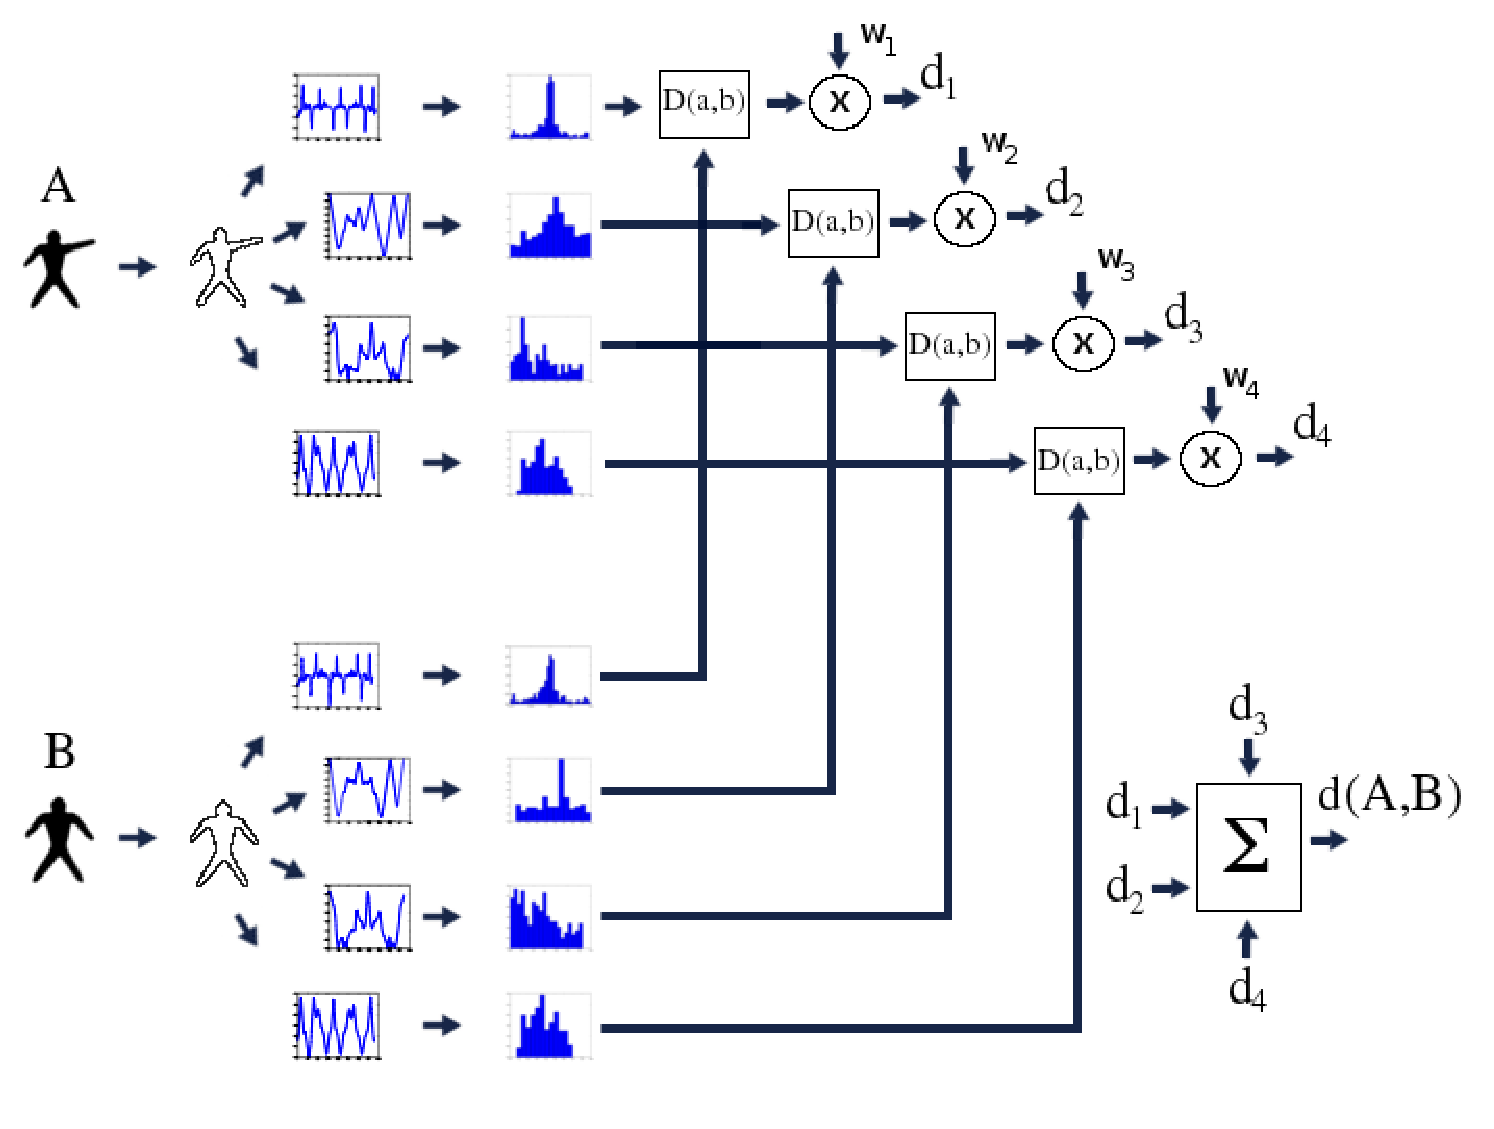
\includegraphics[width=0.85\textwidth]{figura_metodo.eps}
\end{figure}

%Isso porque embora duas formas estejam numa mesma classe, estas podem ter variações substanciais em suas características de baixo nível, e mesmo assim serem consideradas similares apesar da distância entre as mesmas ser significativas.

\section{Medidas de divergência}

Se $X\text{ e }Y$ são variáveis aleatórias discretas, ambas podendo assumir um conjunto de valores $\chi \in \{x_{1},x_{2},x_{3},\ldots,x_{n}\}$, então suas densidades de probabilidade de massa são $p = (p_{1},p_{2},\ldots,p_{n})$ e $q = (q_{1},q_{2},\ldots,q_{n})$ respectivamente, aonde $p_i = Pr(X = x_{i})$ e $q_i = Pr(Y = x_{i})$.    

Com base nessa definição este capítulo apresenta alguns dos divergentes encontrados na literatura. 

\subsection{Divergente de Kullback-Leibler}
O divergente de Kullback-Leibler (KL), também conhecido como entropia relativa, é definido pela seguinte equação:

\begin{equation} \label{eq:kl}
D_{KL}(p,q) = \sum\limits_{i = 1}^{n} p_{i}\log{\frac{p_{i}}{q_{i}}}\text{.}
\end{equation}

Essa medida de divergência não corresponde a uma métrica de distância por não ser simétrica e por não respeitar a propriedade de desigualdade triangular. No entanto demonstra-se que a mesma é sempre positiva, sendo igual a zero se e somente se $p = q$. Outra característica importante do divergente de KL é que seu valor não apresenta um limite superior. Isso porque se, para algum valor de $i$, $p_{i} = 0$ e $q{i} \neq 0$, $D_{KL}(p,q) \to \infty$.

O divergente de KL é de grande importância na teoria da informação. A informação mútua, que é um caso particular do divergente de KL, é uma quantidade definida na teoria da informação como a  medida da capacidade de um canal de comunicação. Ademais, este divergente é empregado em aplicações de comunicação, na seleção de sinais.  

\subsection{Divergente de Jensen-Shannon}

Construído a partir do divergente de Kullback-Leibler, o divergente de Jensen-Shannon é dado por: 

$D_{JS}(p,q) =\frac{1}{2}(D_{KL}(p,h)+D_{KL}(q,h))$, sendo $h = \frac{p+q}{2}$

Embora apresente a propriedade de simetria, este divergente não respeita a propriedade de desigualdade triangular. A faixa de valores que este pode assumir é delimitada entre $0$ e $1$ no caso de o logaritmo da Equação \ref{eq:kl} ser na base $2$. 

\subsection{Patrick Fisher}

Este divergente foi originalmente proposto em \citeonline{1054354} como uma métrica de distância entre distribuições de probabilidade. No referido trabalho, este é utilizado como uma função custo a ser maximizada na seleção não paramétrica de características.

Em \cite{662771}, o divergente de Patrick-Fisher é utilizado para o reconhecimento de padrões como uma função custo a ser otimizada num método não paramétrico de obtenção de um discriminante linear.  

$D_{PF}(p,q) = \sqrt{\sum\limits_{i=1}^{n}{(p_i-q_i)}^2}$

\section{Chi-square}
$D_{CS}(p,q)= \sum\limits_{i = 1}^{n}{\frac{(p_{i}-h_{i})^2}{h_{i}}}$, sendo $h_{i} = \frac{p_{i} + g_{i}}{2}$

\begin{figure}[h!]
  \caption{\label{fig:graph2} Gráficos ilustrando os valores das divergências entre as distribuições de probabilidade de massa $(p\quad1-p)\text{, } p \in [0,1]$ e $(0,5\quad0,5)$.}
  \centering
  \includegraphics[width=0.75\textwidth]{graph2.eps}
\end{figure}

\subsection{Divergente de Rényi}
O divergente de Rényi generaliza algumas das medidas de divergência apresentadas até então.

$D_{\alpha}(p,q) =\frac{1}{\alpha-1}\log{\sum\limits_{i = 1}^{n}{p_i^{\alpha}q_i^{1-\alpha}}}$

\subsection{Chernoff}
$\displaystyle D_C(p,q) = - \min_{0<\alpha<1}{log{\sum\limits_{i=1}^{n}{p_i^{\alpha}q_i^{1-\alpha}}}}$

\subsection{Bhattacharyya}
$D_{B}(p,q) = -2log{\sum\limits_{i = 1}^{n}{\sqrt{p_{i}q_{i}}}}$

\subsection{Hellinger}
$D_{H}=\frac{1}{\sqrt{2}}\sqrt{\sum\limits_{i = 1}^{n}{(\sqrt{p_{i}}-\sqrt{q_{i}})^2}}$


\section{Resultados Experimentais}

\begin{table*}
\centering
\caption{\label{tab:Kimia} Total de acertos por classe e por posição, nos experimentos \emph{CBIR}, com a distância de Chernoff.}
\begin{tabular}{l| r r r r r r r r r r r}
\hline
&\multicolumn{11}{l}{nth nearest match} \\
\cline{2-12}
Classe&1&2&3&4&5&6&7&8&9&10&11 \\
 \hline
Peixes&11&11&11&11&9&5&8&3&7&5&5\\
Coelhos&11&11&11&11&11&11&11&11&11&11&7\\ 
Aviões&11&10&8&8&7&7&7&5&2&1&1\\
ETs&11&11&11&11&11&11&11&11&8&7&5\\
Ferramentas&11&8&7&10&3&9&9&5&7&9&9\\
Mãos&11&11&11&11&11&11&11&11&11&9&7\\
humanos&11&11&11&11&11&11&11&11&11&11&11\\
Quadrupedes&11&11&9&8&8&7&8&3&5&8&4\\
Arraias&11&11&11&11&11&11&11&10&11&9&7\\
\hline
Total&99&95&90&92&82&83&87&70&73&70&56\\
\hline
\end{tabular}
\end{table*}

\begin{table*}
\centering
\caption{\label{tab:Kimia} Total de acertos por classe e por posição, nos experimentos \emph{CBIR}, com a distância de Chi-square.}
\begin{tabular}{l| r r r r r r r r r r r}
\hline
&\multicolumn{11}{l}{nth nearest match} \\
\cline{2-12}
Classe&1&2&3&4&5&6&7&8&9&10&11 \\
 \hline
Peixes&11&11&11&10&10&8&7&9&4&4&3\\
Coelhos&11&10&10&10&10&10&10&10&10&8&1\\ 
Aviões&11&11&11&9&9&9&8&5&2&2&2\\
ETs&11&11&11&10&11&10&11&10&10&8&7\\
Ferramentas&11&11&11&11&11&11&11&11&10&11& 11\\
Mãos&11&11&11&11&11&11&11&11&11&11&9\\
humanos&11&11&11&11&11&11&11&11&11&11&11\\
Quadrupedes&11&11&6&9&8&7&7&5&7&7&4\\
Arraias&11&11&11&11&11&11&11&10&11&11&10\\
\hline
Total&99&98&93&92&92&88&87&82&76&73&58\\
\hline
\end{tabular}
\end{table*}

\begin{table*}
\centering
\caption{\label{tab:Kimia} Total de acertos por classe e por posição, nos experimentos \emph{CBIR}, com a distância de Hellinger.}
\begin{tabular}{l| r r r r r r r r r r r}
\hline
&\multicolumn{11}{l}{nth nearest match} \\
\cline{2-12}
Classe&1&2&3&4&5&6&7&8&9&10&11 \\
 \hline
Peixes&11&11&11&10&10&9&5&8&8&2&2\\
Coelhos&11&11&11&11&11&10&10&10&11&8&2\\ 
Aviões&11&11&11&10&9&11&9&8&1&1&0\\
ETs&11&11&11&11&10&11&10&11&11&7&4\\
Ferramentas&11&11&11&11&11&11&11&10&11&11& 10\\
Mãos&11&11&11&11&11&11&11&11&11&11&8\\
humanos&11&11&11&11&11&11&11&11&11&11&11\\
Quadrupedes&11&11&7&9&6&6&5&7&9&5&4\\
Arraias&11&11&11&11&11&11&11&11&11&10&9\\
\hline
Total&99&99&95&95&90&91&83&87&84&66&50\\
\hline
\end{tabular}
\end{table*}

\begin{table*}
\centering
\caption{\label{tab:Kimia} Total de acertos por classe e por posição, nos experimentos \emph{CBIR}, com a distância Jensen-Shannon.}
\begin{tabular}{l| r r r r r r r r r r r}
\hline
&\multicolumn{11}{l}{nth nearest match} \\
\cline{2-12}
Classe&1&2&3&4&5&6&7&8&9&10&11 \\
 \hline
Peixes&11&11&11&10&10&8&7&7&7&4&1\\
Coelhos&11&10&10&10&10&10&10&10&9&8&2\\ 
Aviões&11&11&10&10&9&8&8&6&3&1&1\\
ETs&11&11&11&10&11&10&10&11&9&8&5\\
Ferramentas&11&11&11&11&11&11&11&11&10&11& 11\\
Mãos&11&11&11&11&11&11&11&11&11&11&9\\
humanos&11&11&11&11&11&11&11&11&11&11&11\\
Quadrupedes&11&11&7&8&8&5&3&8&8&7&4\\
Arraias&11&11&11&11&11&11&11&11&10&11&10\\
\hline
Total&99&98&93&92&92&85&82&86&78&72&54\\
\hline
\end{tabular}
\end{table*}

\begin{table*}
\centering
\caption{\label{tab:Kimia} Total de acertos por classe e por posição, nos experimentos \emph{CBIR}, com a distância Patrick-Fisher.}
\begin{tabular}{l| r r r r r r r r r r r}
\hline
&\multicolumn{11}{l}{nth nearest match} \\
\cline{2-12}
Classe&1&2&3&4&5&6&7&8&9&10&11 \\
 \hline
Peixes&11&11&11&10&10&9&8&5&4&1&1\\
Coelhos&11&9&9&9&9&10&10&9&7&4&4\\ 
Aviões&11&11&10&9&8&9&7&5&3&2&2\\
ETs&11&11&11&10&9&9&9&9&7&6&5\\
Ferramentas&11&10&11&11&11&10&11&11&7&9  &7\\
Mãos&11&11&11&11&11&11&11&11&11&11&9\\
humanos&11&11&11&11&11&11&11&11&11&11&10\\
Quadrupedes&11&11&8&9&8&7&5&5&7&6&6\\
Arraias&11&11&11&11&11&11&10&10&11&9&6\\
\hline
Total&99&96&93&91&88&87&82&76&68&59&50\\
\hline
\end{tabular}
\end{table*}


\begin{figure}[h!]
  \caption{\label{fig:graph1} Gráficos precisão/revocação para diferentes combinações de assinaturas. Resultados obtidos nos experimentos de recuperação de formas pelo conteúdo, com a base de imagens MPEG-7, empregando como medida de similaridade o divergente de Hellinger. }
  \centering
  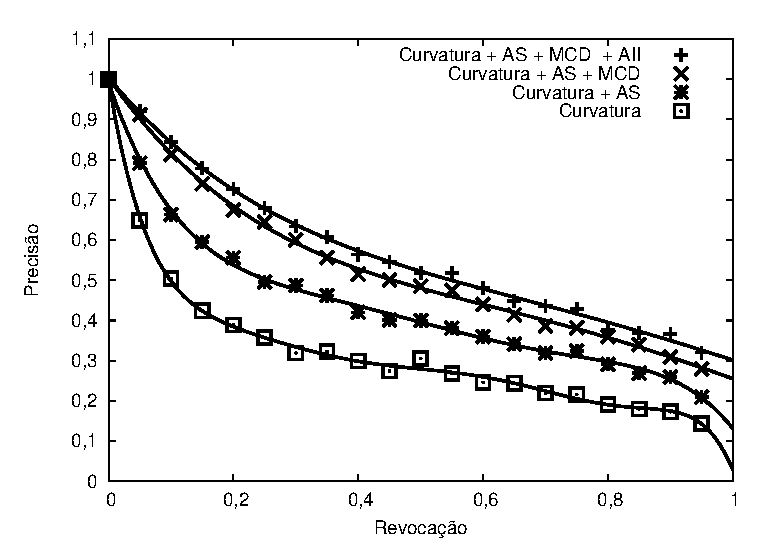
\includegraphics[width=0.75\textwidth]{graph1.eps}
\end{figure}

\color{red}
\chapter{Metodologias propostas}

\section{Descritor entropia multiescala da curvatura}


\section{Experimentos CBIR}

A Figura \ref{fig:metodo_cbir} ilustra o método experimental empregado na avaliação do desempenho dos descritores em experimentos de recuperação de formas pelo conteúdo.

Primeiramente é realizada a extração de características numa base de formas binárias com o método de descrição sob avaliação. O mesmo processo de extração de características é aplicado a uma forma protótipo. Desse processo resulta uma base de vetores de características. 

Avaliando-se o grau de similaridade entre a representação vetorial da forma protótipo e as representações vetoriais de cada uma das formas pertencentes a base de formas tem-se como resultado do experimento as formas recuperadas na ordem decrescente de similaridade ao protótipo. Todo esse processo é repetido para cada forma da base de formas tomada como protótipo.

\begin{figure}[h!]
  \caption{\label{fig:metodo_cbir} Metodologia empregada para os experimentos de recuperação de formas pelo conteúdo.}
  \centering
  \includegraphics[width=0.55\textwidth]{Metodologia1.jpg}
\end{figure}

Na avaliação de desempenho do experimento é calculado o número total de acertos por classe e por posição do rank. Essa medida contabiliza, para cada classe de formas, o número total de ocorrências que pertencentes a mesma classe do protótipo em cada posição do rank.   


 

\section{Fusão de características}

Conforme ilustra a Figura \ref{fig:features1} contruímos três bases de dados de vetores de características multiescala a partir das formas da base da Figura \ref{fig:db1}. A aplicação da técnica PCA às características multiescala possibilita obter como saída vetores de componentes descorrelacionadas e de máxima variância (citar). 

\begin{figure}[h!]
  \caption{\label{fig:features1} Metodologia que emprega a técnicas \emph{PCA} para obtenção de um descritor híbrido através da fusão de descritores multiescala.}
  \centering
  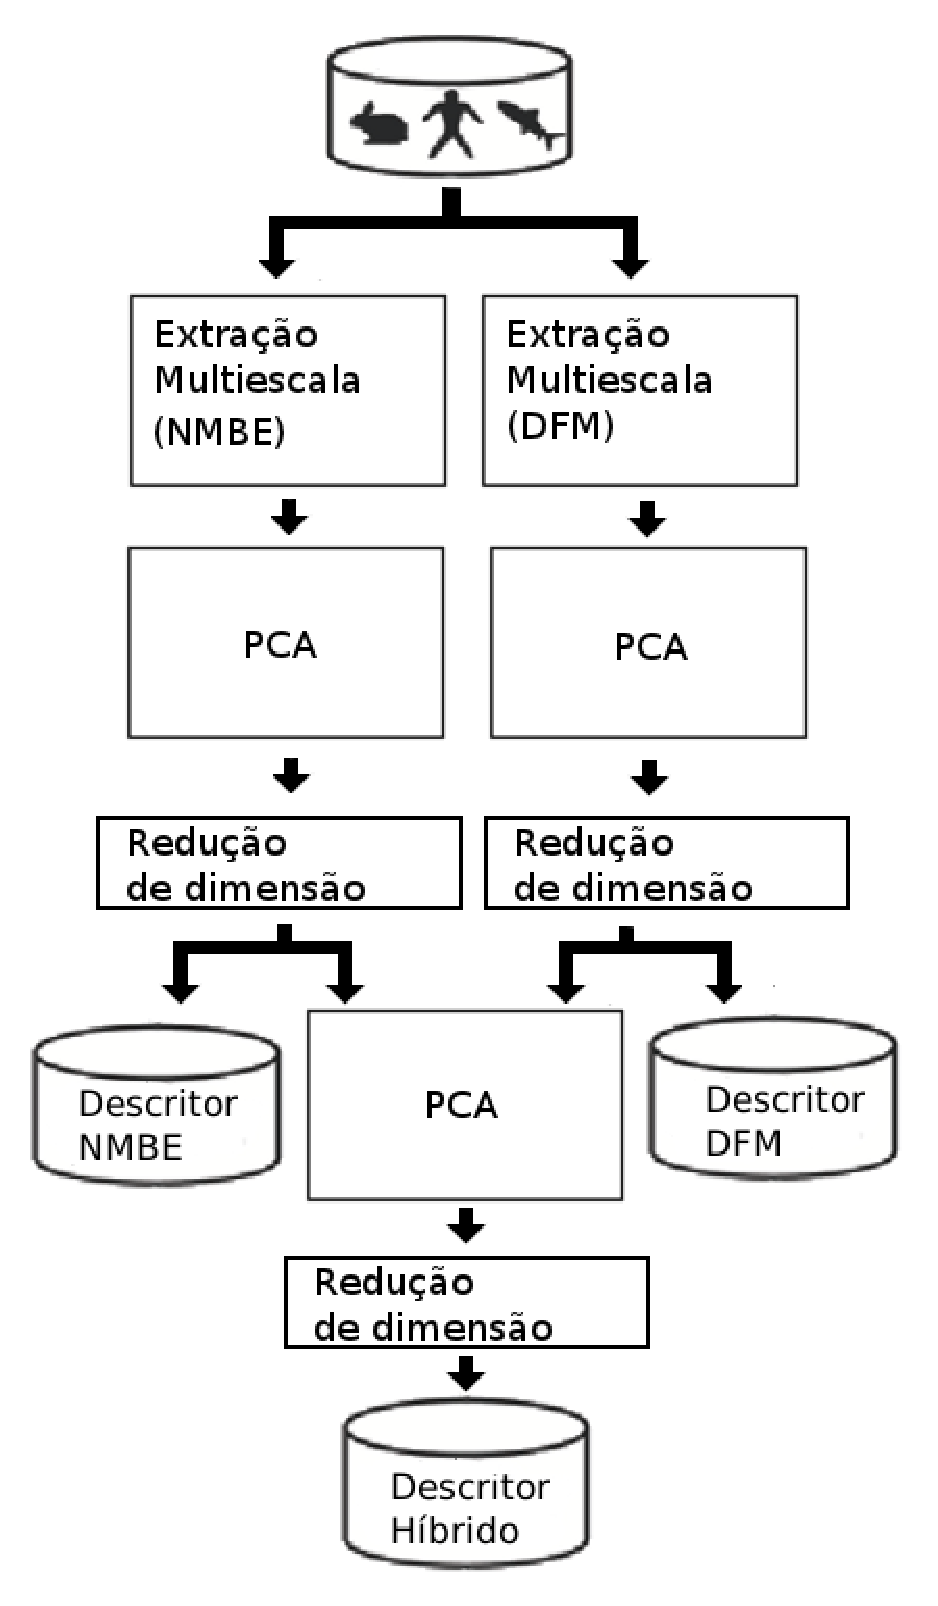
\includegraphics[width=0.45\textwidth]{features1.eps}
\end{figure}

\begin{figure}[h!]
  \caption{\label{fig:acuracia} Acurácia média por classe aferida nos experimentos de recuperação de formas pelo conteúdo, com a base Kimia-99, para os descritores (a) Dimensão fractal multiescala; (b) Energia de dobramento multiescala.}
  \centering
  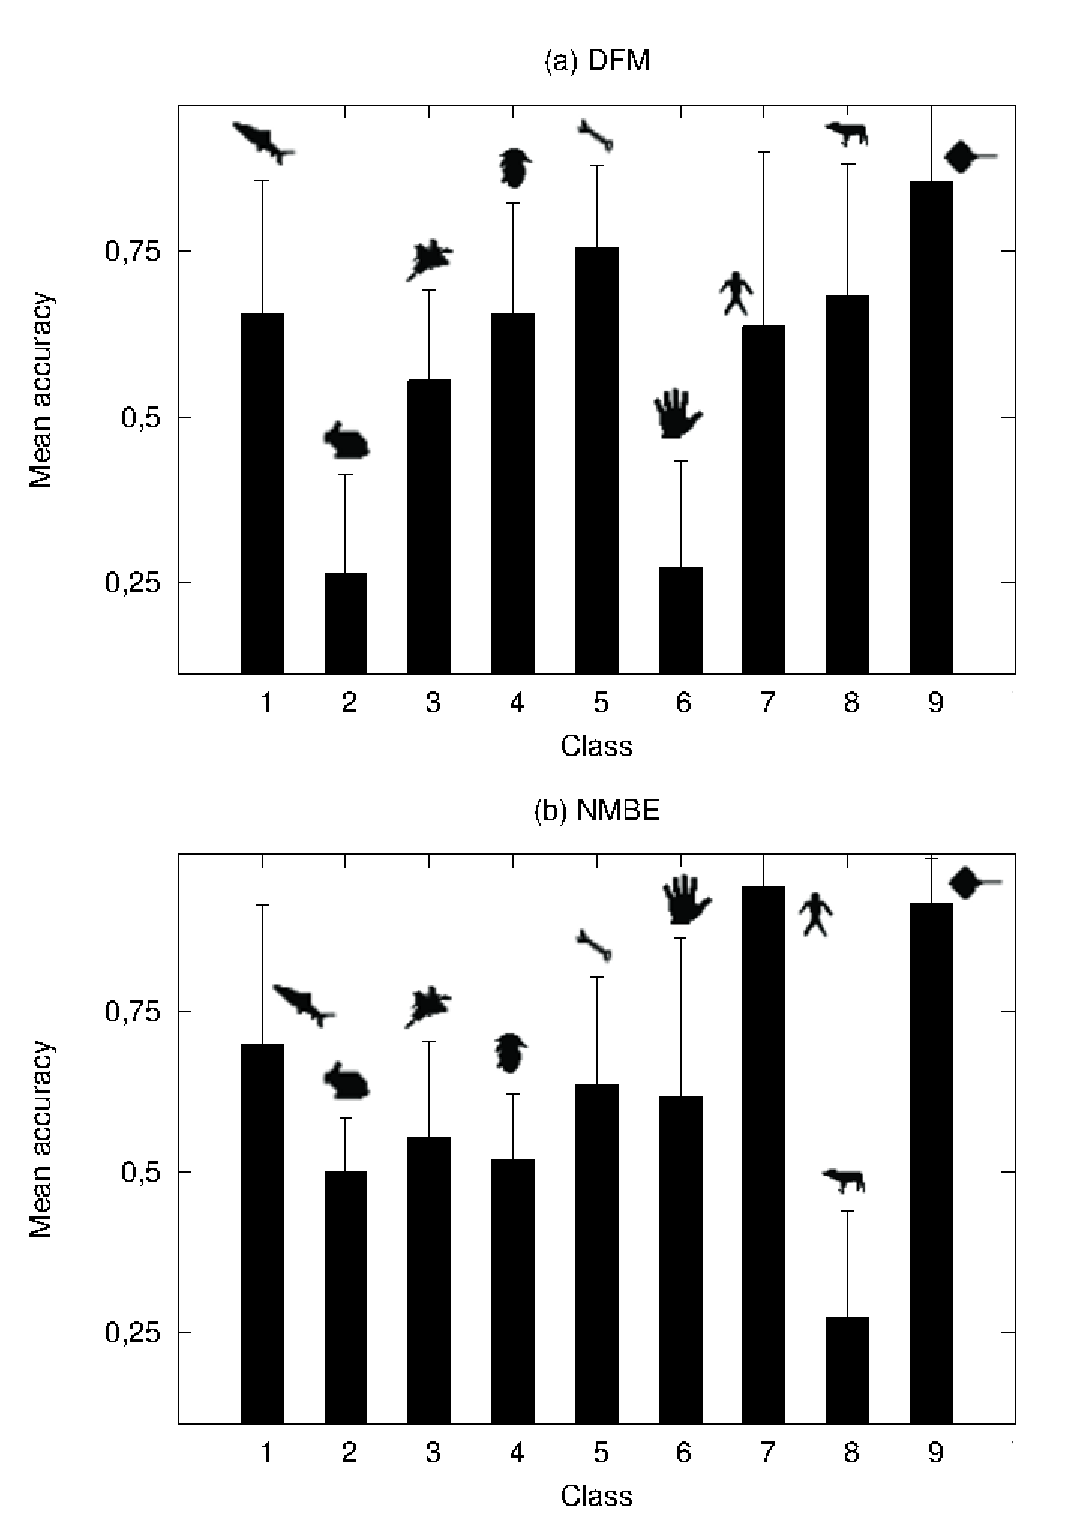
\includegraphics[width=0.75\textwidth]{resultado_acuracia.eps}
\end{figure}


\color{black}
\begin{comment}
\section{Bases de imagens}
\end{comment}
\begin{comment}
\begin{figure}
\centering
\caption{\label{Met:1}Metodologia 1}
\includegraphics[width=0.5\textwidth]{Metodologia1.eps}
\end{figure}

\begin{figure}
\centering
\caption{\label{Met:2}Metodologia 2}
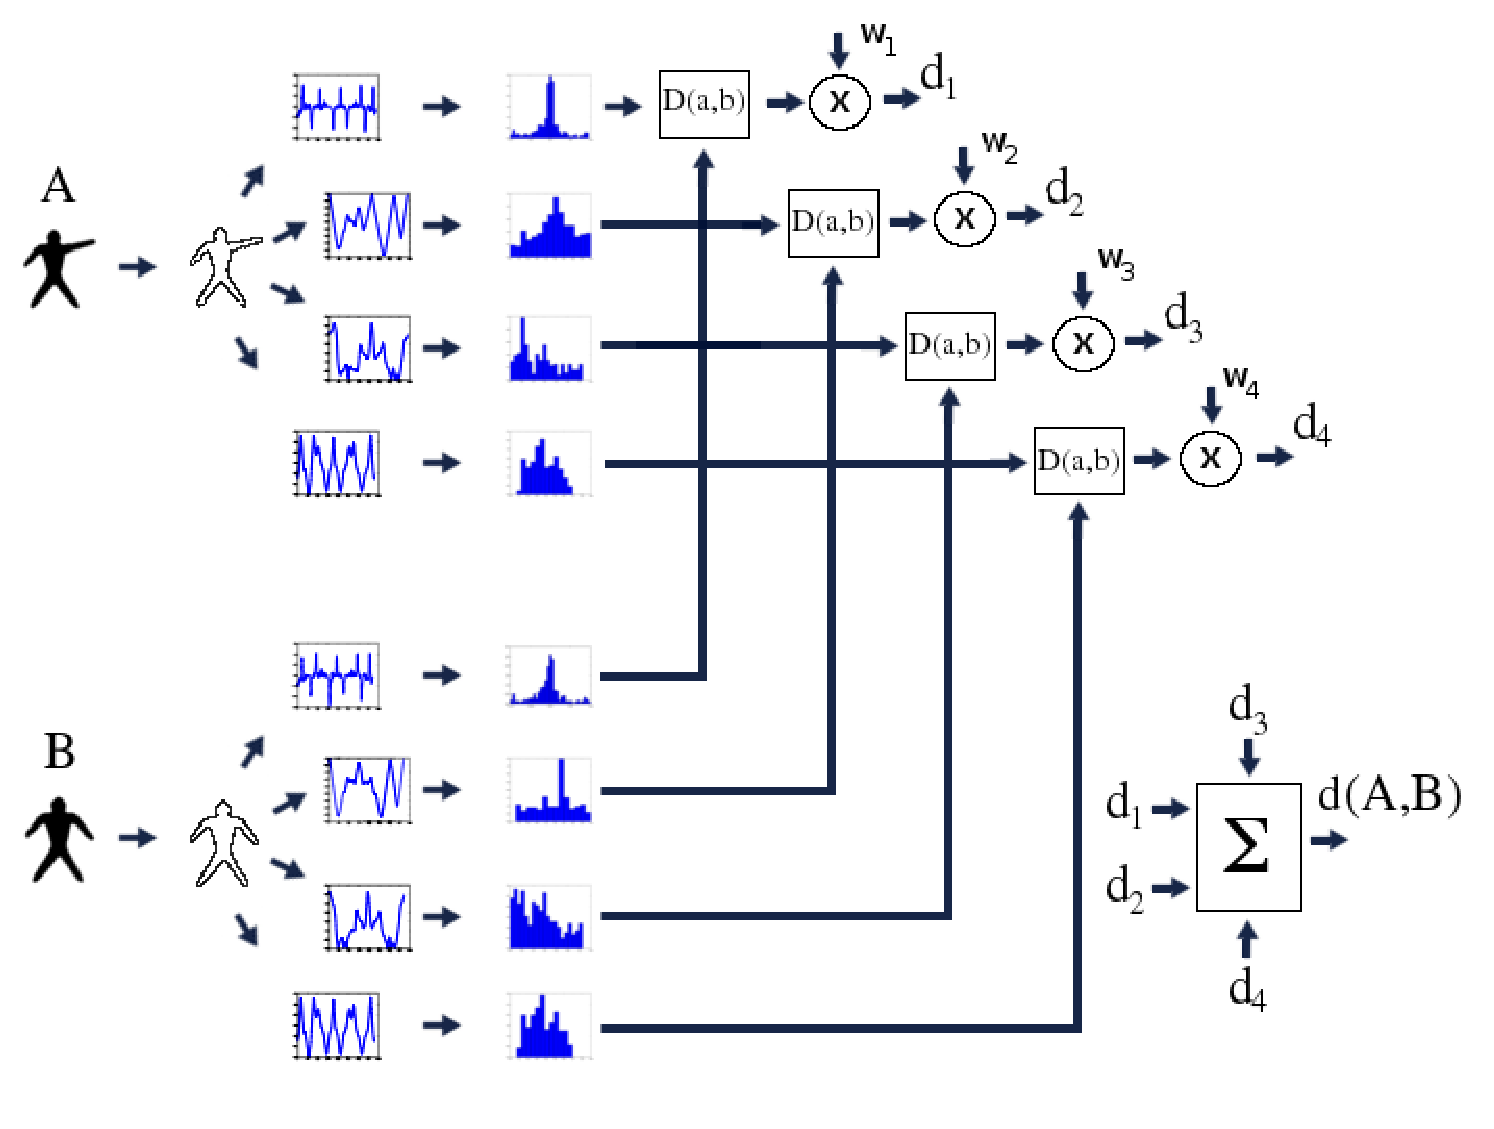
\includegraphics[width=\textwidth]{figura_metodo.eps}
\end{figure}
\end{comment}